\documentclass{article}
\usepackage{amsmath, amssymb, graphicx, subfigure, algorithmic, color}

\author{Mitchell Koch, Justin Huang}
\title{Learning Relation Entailment Graphs\\CSE 515 Final Report}
\date{Friday, June 14, 2013}

\begin{document}
\maketitle

\begin{abstract}
Can learning relation entailment graphs based on WordNet or Bayes net
structure learning improve relation query performance?
\end{abstract}

\section{Introduction and Motivation}

Open IE~\cite{Etzioni:2008:OIE:1409360.1409378}

previous relation entailment
work~\cite{Berant:2012:LER:2122944.2122947, berant2011global}, on work in relation
extraction using matrix factorization~\cite{riedel13relation}, 

as well as on related work in probabilistic modeling of relations
between entities~\cite{TaskarWAK03, Taskar:2002:DPM:2073876.2073934}.

Freebase using distant supervision as in~\cite{HoffmannZLZW11}

\subsection{Database Query Task}

Given a query for relation $R$ with arguments $X$ and $Y$, we expand the query to include all entailing relations. Given an original query $R(X, Y)$, it is expanded to $R^\prime(X,Y)$ for all $R^\prime$ such that there is an edge from $R^\prime$ to $R$ in the entailment graph. This process is shown in Figure~\ref{query-expansion}. 

\begin{figure}[h]
\begin{center}
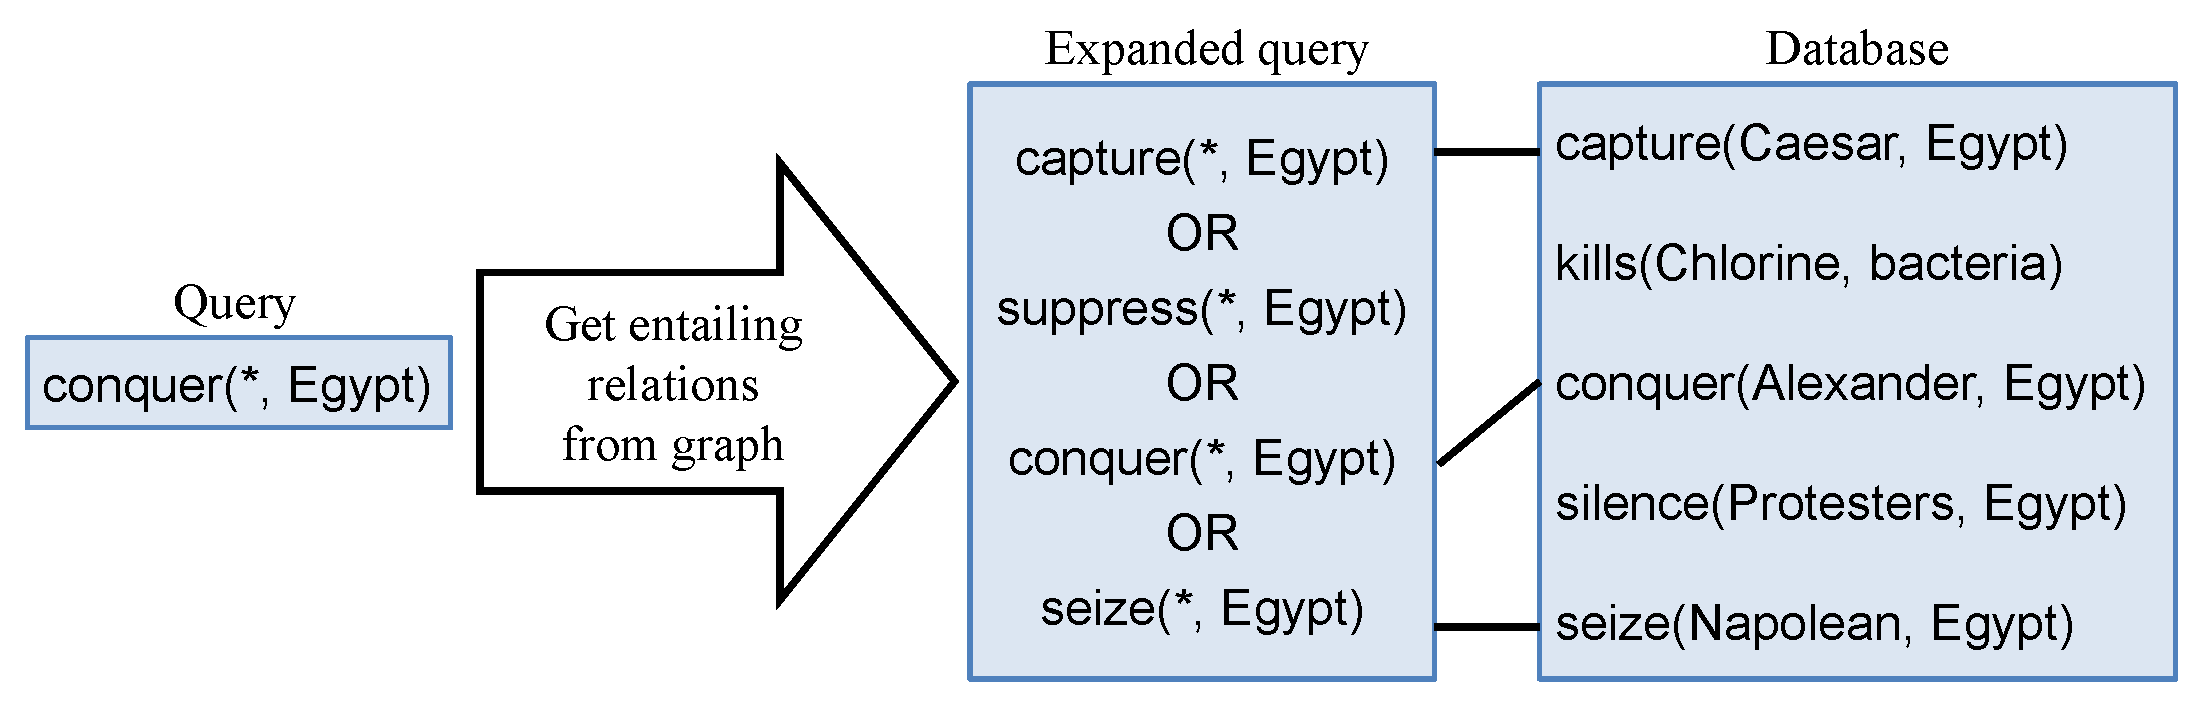
\includegraphics[width=1.0\textwidth]{figures/query-expansion.pdf}
\end{center}
\caption{An example of a query being expanded.}\label{query-expansion}
\end{figure}

\section{Methods and Algorithms}

\subsection{Constraints on WordNet}

WordNet~\cite{fellbaum98wordnet} is a hand-crafted resource that
distinguishes between different word senses, and provides synonyms and
entailments between them. We denote a word net sense with a number where \textit{\#1} is the most common. For example \textit{note\#4} is the fourth most common sense of ``note,'' which means ``to write down''. Each WordNet sense has its sense number, a count indicating how often that sense is used, and a probability, which is the count divided by the sum of counts for all senses of the same word.

The challenge in using WordNet for relation entailment is that we need to determine what sense to use. Given the verb ``take,'' is it \textit{take\#21} (take by force) or \textit{take\#2} (take time)?

We follow the following steps for our method.

\begin{enumerate}
\item Assume a string can be any WordNet sense (``take'' = \textit{take\#1}, \textit{take\#2}, \ldots, \textit{take\#42})
\item Attempt the database query task using all possible entailments.
\item Label results as correct/incorrect
\item Split results into train / test sets, gather features of the path taken through the entailment graph that connected the result to the query.
\item Train a model of the probability that the path is correct given features of the path using
logistic regression.
\item Evaluate the model on the test set.
\end{enumerate}

Our features for a path in the entailment graph are as follows.
\begin{enumerate}
\item Path length
\item Average sense number
\item Average WordNet probability
\item Maximum sense number
\item Minimum WordNet probability
\end{enumerate}

% TODO give justifications and explanations for the features

\begin{figure}[h]
\begin{center}
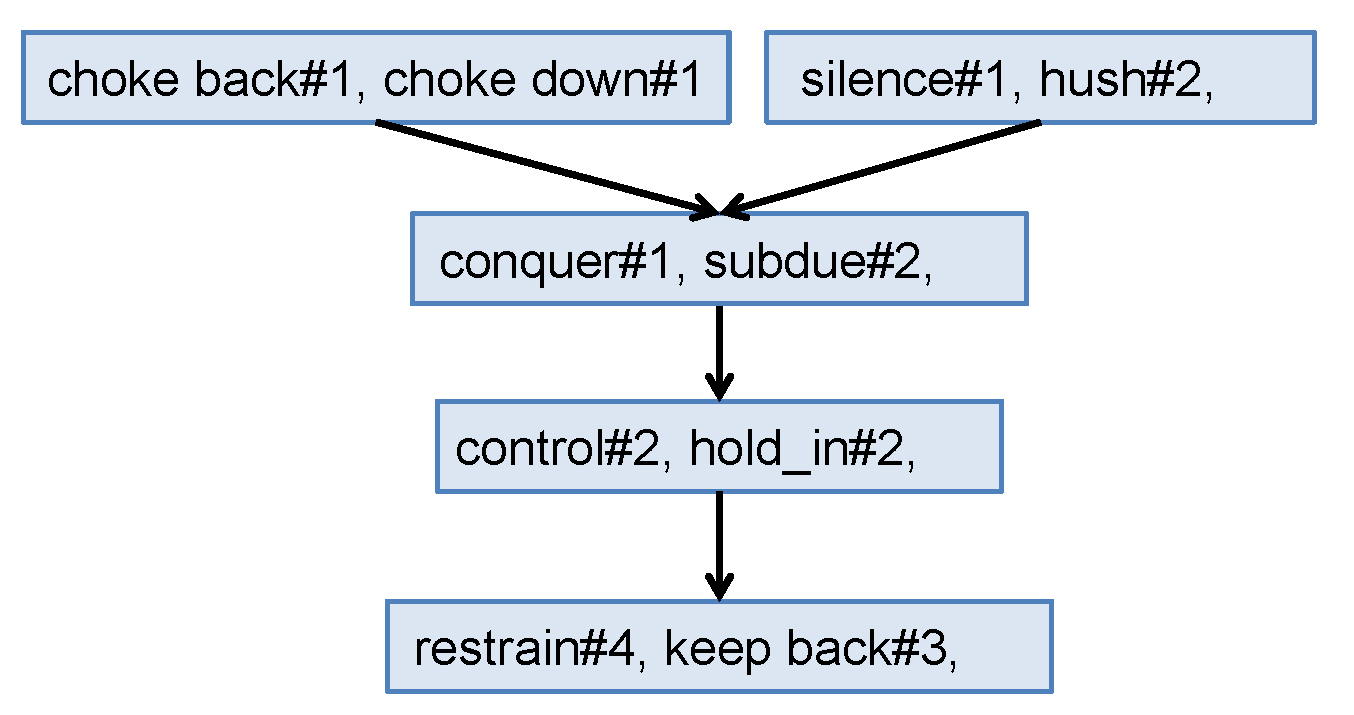
\includegraphics[width=0.6\textwidth]{figures/wordnet-graph.pdf}
\end{center}
\caption{Component of the WordNet entailment graph with the first sense of conquer, \textit{conquer\#1}. Boxes represent synonym sets, arrows represent entailments.}\label{wordnet-graph}
\end{figure}


\begin{figure}[h]
\begin{center}
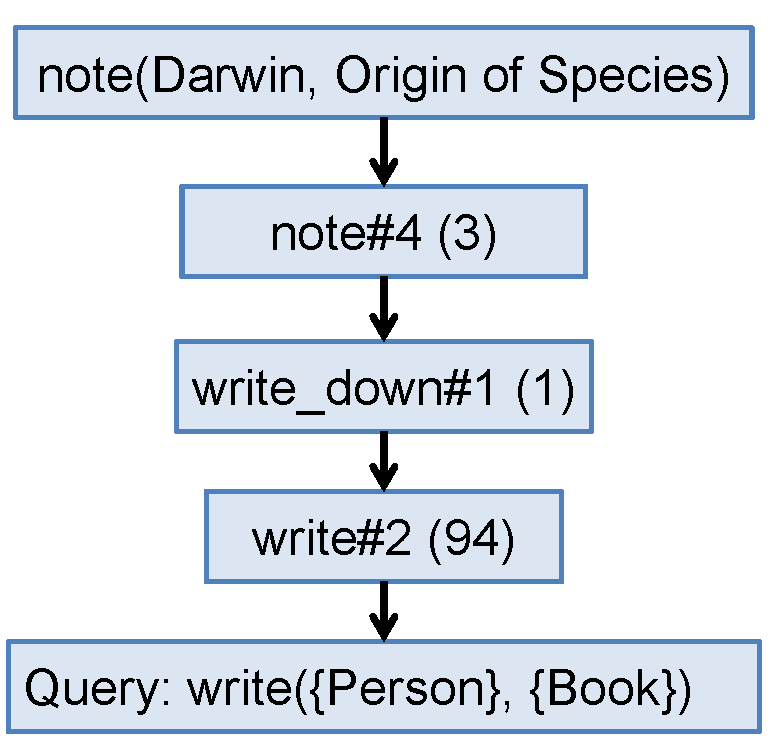
\includegraphics[width=0.4\textwidth]{figures/example-path.pdf}
\end{center}
\caption{Example path in entailment graph}\label{example-path}
\end{figure}


\subsection{Bayesian Network Structure Learning}

\begin{figure}[h]
\begin{center}
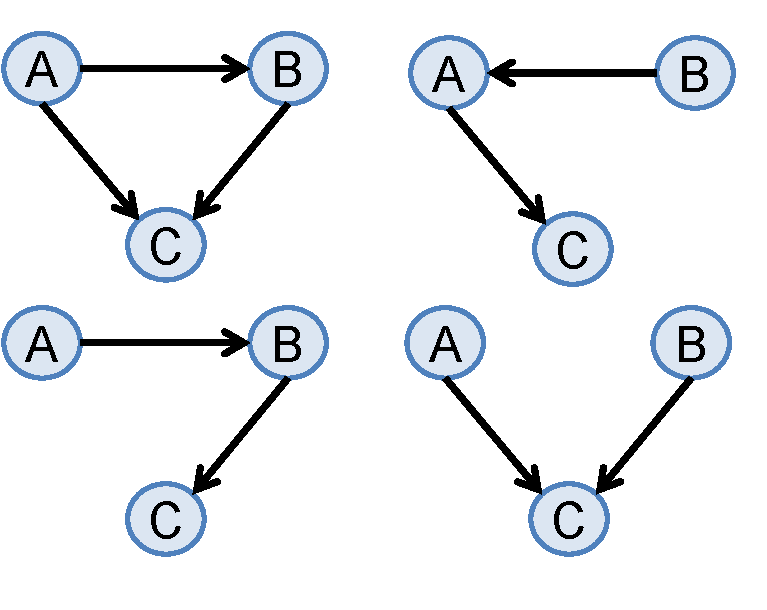
\includegraphics[width=0.4\textwidth]{figures/example-net-structures.pdf}
\end{center}
\caption{Examples of possible network structures}\label{example-net-structures}
\end{figure}


\section{Experiments and Results}

\section{Discussion and Conclusion}


\bibliographystyle{abbrv}
\bibliography{bib}

\end{document}
